% =============================================================================
% Chuong 2: Kien thuc va cong nghe nen tang
% =============================================================================
% Cach dung tren Overleaf:
%   1. Tai thu muc thesis/ (hoac sao chep macros.tex, refs.bib, chapters/ch2.tex
%      va figures/ch2/*.png) vao du an Overleaf.
%   2. Trong main.tex:
%        \input{macros}
%        ...
%        \include{chapters/ch2}
%        ...
%        \bibliographystyle{IEEEtran}
%        \bibliography{refs}
%
% Cac nhan lien chuong duoc tham chieu tu Chuong 2 (dat dung \label o cac
% chuong tuong ung de \ref tu dong hien so):
%   Chuong: ch:de-xuat, ch:thuc-nghiem, ch:platform, ch:thao-luan
%   Chuong 4: sec:ch4-detector, sec:ch4-ctav, sec:ch4-bm25, sec:ch4-c1,
%             sec:ch4-policy, sec:ch4-c4, sec:ch4-judge, sec:ch4-rca,
%             sec:ch4-grouping, sec:ch4-propagation, sec:ch4-report, sec:ch4-impl
%   Chuong 5: sec:ch5-hypotheses, sec:ch5-data, sec:ch5-metrics, sec:ch5-val,
%             sec:ch5-h1, sec:ch5-c5, sec:ch5-h4, sec:ch5-budget, sec:ch5-rca,
%             tab:h0-h5
%   Chuong 7: sec:ch7-threats
% =============================================================================

\section{Kiến thức và công nghệ nền tảng}
\label{ch:nen-tang}

Chương này trình bày các khái niệm và công nghệ mà phần đề xuất (Chương~\ref{ch:de-xuat}) và phần thực nghiệm (Chương~\ref{ch:thuc-nghiem}) dựa vào. Nội dung đi theo đúng thứ tự xử lý của hệ thống. Mục~\ref{sec:ch2-du-lieu} mô tả dữ liệu quan sát của hệ microservice và bộ dữ liệu Nezha. Mục~\ref{sec:ch2-phat-hien} nói về phát hiện bất thường và hiện tượng quá tải cảnh báo. Mục~\ref{sec:ch2-truy-xuat} trình bày các cách truy xuất bằng chứng từ log và trace: \term{BM25}{BM25}, đồ thị phụ thuộc service và cách hợp nhất chúng. Mục~\ref{sec:ch2-judge} giải thích cơ chế dùng mô hình ngôn ngữ lớn làm bộ thẩm định và các rủi ro của nó, Mục~\ref{sec:ch2-rca} giới thiệu bài toán phân tích nguyên nhân gốc. Mục~\ref{sec:ch2-danh-gia} và Mục~\ref{sec:ch2-dang-ky} định nghĩa chỉ số, kiểm định thống kê và nguyên tắc đăng ký giả thuyết trước. Mục~\ref{sec:ch2-cong-nghe} giới thiệu các công nghệ dùng để hiện thực hệ thống, và Mục~\ref{sec:ch2-ket-chuong} tổng kết.

% -----------------------------------------------------------------------------
\subsection{Dữ liệu quan sát trên hệ microservice}
\label{sec:ch2-du-lieu}

Mục này xác định đơn vị dữ liệu mà toàn bộ đề tài làm việc trên đó: ba loại tín hiệu quan sát, cách cắt chúng thành cửa sổ, và bộ dữ liệu có nhãn dùng để đánh giá.

\subsubsection{Metric, log, trace và cửa sổ trượt}
\label{sec:ch2-tin-hieu}

Một hệ microservice gồm nhiều service nhỏ, mỗi service chạy trên một hoặc nhiều pod và gọi nhau qua mạng. Khả năng quan sát (\emph{observability}) của hệ dựa trên ba loại tín hiệu, tóm tắt ở Bảng~\ref{tab:ch2-tin-hieu}. \textbf{Metric} là chuỗi thời gian số đo định kỳ cho từng pod, như mức dùng CPU, bộ nhớ, lưu lượng mạng hay độ trễ phân vị. Độ trễ phân vị P$k$ là mức độ trễ mà $k\%$ request trong chu kỳ đo không vượt quá: P99 bằng $500$~ms nghĩa là $99\%$ request hoàn tất trong $500$~ms, nên P95 và P99 phản ánh phần đuôi chậm mà độ trễ trung bình che mất. Khái niệm phân vị này cũng là cơ sở của ngưỡng nền $p_{90}$ mà cơ chế neo bằng chứng \comp{C3} dùng (Mục~\ref{sec:ch4-policy}). \textbf{Log} là các dòng văn bản do service ghi ra, thường kèm mức nghiêm trọng (\code{INFO}, \code{WARN}, \code{ERROR}). \textbf{Trace} ghi lại đường đi của một request qua nhiều service. Mỗi bước trên đường đi là một \textbf{span}, có định danh \code{SpanID}, định danh span cha \code{ParentID}, tên thao tác và thời lượng. Quan hệ cha--con giữa các span cho biết service nào gọi service nào.

\begin{table}[H]
  \centering
  \caption{Ba loại tín hiệu quan sát trên Nezha và vai trò của chúng trong đề tài.}
  \label{tab:ch2-tin-hieu}
  \tblfont
  \tblsetup
  \renewcommand{\arraystretch}{1.35}
  \setlength{\tabcolsep}{6pt}
  \begin{tabularx}{\linewidth}{|l|>{\hsize=0.70\hsize}Y|>{\hsize=1.45\hsize}Y|>{\hsize=0.85\hsize}Y|}
    \hline
    \rowcolor{gray!15}
    \textbf{Tín hiệu} & \textbf{Dạng dữ liệu trên Nezha} & \textbf{Trường chính} & \textbf{Vai trò trong đề tài} \\
    \hline
    Metric & CSV theo pod, một mẫu mỗi 60~s & 19 chỉ số: CPU, bộ nhớ, syscall, mạng vào/ra, độ trễ client/server ở phân vị 90/95/99 (P90/P95/P99), workload, tỉ lệ thành công, tài nguyên node & Đầu vào của bộ phát hiện bất thường \\
    \hline
    Log & CSV theo phút & thời điểm, pod, \code{TraceID}, \code{SpanID}, nội dung (kèm mức nghiêm trọng) & Bằng chứng văn bản cho judge \\
    \hline
    Trace & CSV theo phút & \code{TraceID}, \code{SpanID}, \code{ParentID}, pod, tên thao tác, thời điểm bắt đầu/kết thúc, thời lượng & Bằng chứng về độ trễ; nguồn dựng đồ thị phụ thuộc service \\
    \hline
  \end{tabularx}
\end{table}


Đề tài dùng metric để \emph{phát hiện} và dùng log, trace làm \emph{bằng chứng}. Cách chia vai này bám theo cách dữ liệu được ghi: metric có ở mọi thời điểm, còn log và trace dày đặc và cần được chọn lọc trước khi đưa cho một mô hình đọc.

\textbf{Cửa sổ. (Window)} Đơn vị phân tích của hệ là \textbf{cửa sổ}: một mẫu metric của một pod dài $60\,\text{s}$ (chu kỳ lấy mẫu của Nezha), có định danh tất định từ service, pod và thời điểm bắt đầu. Một cửa sổ được gán nhãn \textbf{có sự cố} nếu thuộc đúng pod bị tiêm lỗi và rơi vào khoảng $[t_{\mathrm{inject}} - 60\text{ s},\; t_{\mathrm{inject}} + 360\text{ s}]$ (khoảng bảy cửa sổ mỗi lần tiêm, bắt cả dấu hiệu sớm lẫn thời gian lỗi lan); các cửa sổ còn lại là bình thường. Bộ phát hiện không nhìn cửa sổ cô lập mà duy trì bộ đệm trượt ngắn trên cùng pod (Mục~\ref{sec:ch4-detector}), còn bằng chứng log/trace được tìm trong biên $\pm 8$~phút quanh cửa sổ. Định nghĩa cửa sổ và quy tắc nhãn này được dùng thống nhất cho bộ phát hiện ở Chương~\ref{ch:de-xuat} và mọi phép đo ở Chương~\ref{ch:thuc-nghiem}.

\subsubsection{Nezha và nhãn nguyên nhân gốc}
\label{sec:ch2-nezha}

Nezha~\cite{nezha} là bộ dữ liệu quan sát đa phương thức (metric, log, trace) thu từ hai hệ microservice mẫu là \textbf{OnlineBoutique} và \textbf{TrainTicket}, với các lỗi được tiêm có chủ đích (độ trễ mạng, tranh chấp/tiêu thụ CPU, ngoại lệ, giá trị trả về sai). Đề tài dùng bốn ngày dữ liệu gồm $101$ lần tiêm lỗi trên $95.660$ cửa sổ thuộc $103$ pod ($56$ service), trong đó chỉ có $704$ cửa sổ có sự cố ($\approx 0{,}74\%$, tỷ lệ mất cân bằng xấp xỉ $1:135$). Mỗi lần tiêm lỗi ghi rõ pod bị tiêm và ánh xạ được về tên \textbf{service gốc} cho bài toán \term{RCA}{RCA} (Mục~\ref{sec:ch2-hitk}); đề tài sử dụng cột giờ hệ thống (\emph{wall-clock}) nhất quán trên cả bốn ngày.

Để tránh rò rỉ dữ liệu theo sự kiện và thời gian, dữ liệu được chia thành ba tập \splitname{dev}, \splitname{val} và \splitname{test} theo đơn vị \textbf{lần tiêm lỗi} kèm \textbf{vùng đệm $600\,\text{s}$}, giữ nguyên tỷ lệ mất cân bằng tự nhiên. Do Nezha chỉ ghi log và trace quanh các khoảng tiêm lỗi (chỉ khoảng một phần tư cửa sổ bình thường có telemetry), chỉ số chính của nhánh thẩm định được tính trên tập con \textbf{\term{TelemetryWindow}{cửa sổ có telemetry}} (xác định chỉ từ danh sách tệp, không dùng nhãn) nhằm tránh việc bộ thẩm định bác bỏ đúng một cách tầm thường trên vùng trống dữ liệu. Chi tiết kích thước từng split, độ phủ telemetry và rủi ro tính hợp lệ liên quan được trình bày ở Mục~\ref{sec:ch5-data} và Mục~\ref{sec:ch7-hop-le}.

% -----------------------------------------------------------------------------
\subsection{Phát hiện bất thường và quá tải cảnh báo}
\label{sec:ch2-phat-hien}

Mục này giải thích vì sao một bộ phát hiện bất thường trên metric chưa đủ để cảnh báo người vận hành, và giới thiệu Isolation Forest, bộ phát hiện mà đề tài sử dụng.

\subsubsection{Bất thường, khoảng trống ngữ nghĩa và quá tải cảnh báo}
\label{sec:ch2-khoang-trong}

\textbf{Bất thường} (\emph{anomaly}) là điểm dữ liệu lệch khỏi hành vi thường gặp của hệ. Một bộ phát hiện bất thường gán cho mỗi cửa sổ một \textbf{điểm bất thường} và so với một ngưỡng; cửa sổ vượt ngưỡng trở thành \textbf{candidate} cảnh báo. Điểm này chỉ nói rằng số đo khác thường. Nó không nói số đo khác thường \emph{vì sao}, cũng không nói có sự cố hay không. Một đợt tải tăng hợp lệ, một tác vụ định kỳ hay một pod vừa khởi động lại đều có thể làm metric lệch. Khoảng cách giữa ``số đo lệch'' và ``có sự cố cần người xử lý'' được gọi là \textbf{khoảng trống ngữ nghĩa}. Để lấp khoảng trống này, cần ngữ cảnh vận hành mà metric không có, chẳng hạn log lỗi hay trace chậm.

Khi khoảng trống không được lấp, người vận hành nhận rất nhiều cảnh báo, phần lớn là báo động giả. Hiện tượng này gọi là \textbf{quá tải cảnh báo} (\emph{alert fatigue}): người vận hành dần bỏ qua cảnh báo, kể cả cảnh báo thật~\cite{zhao2020alertstorm}. Trên Nezha, mất cân bằng $1:135$ cho thấy vấn đề rõ ràng. Giả sử một bộ phát hiện chỉ báo nhầm 1\% cửa sổ bình thường của \splitname{val} (28.689 cửa sổ). Nó đã sinh khoảng 287 báo động giả, nhiều hơn cả tổng số cửa sổ có sự cố của split này (209). Precision khi đó không thể vượt $209 / (209 + 287) \approx 0{,}42$, kể cả khi bộ phát hiện bắt trọn mọi sự cố.

Đề tài không thay bộ phát hiện. Đề tài thêm một khâu \textbf{thẩm định cảnh báo} đứng sau nó: mỗi candidate được đối chiếu với bằng chứng từ log và trace trước khi chuyển cho người vận hành. Khâu này là \CTAV{} (thẩm định cảnh báo hiệu chỉnh theo bằng chứng đa phương thức), trình bày ở Mục~\ref{sec:ch4-ctav}.

\subsubsection{Isolation Forest}
\label{sec:ch2-iforest}

Isolation Forest~\cite{isof} phát hiện bất thường bằng cách \emph{cô lập} điểm dữ liệu thay vì mô hình hoá dữ liệu bình thường. Ý tưởng là: điểm bất thường ít và khác biệt, nên dễ bị tách riêng bằng vài nhát cắt ngẫu nhiên. Thuật toán dựng nhiều cây cô lập. Mỗi cây chọn ngẫu nhiên một đặc trưng và một giá trị cắt nằm giữa giá trị nhỏ nhất và lớn nhất của đặc trưng đó, rồi chia đệ quy cho đến khi mỗi điểm nằm riêng một lá. Độ dài đường đi $h(x)$ từ gốc tới lá chứa điểm $x$ càng ngắn thì $x$ càng dễ cô lập, tức càng bất thường. Điểm bất thường chuẩn hoá của $x$ trên tập huấn luyện cỡ $n$ được định nghĩa ở Phương trình~\eqref{eq:ch2-iforest}:
\begin{align}
  s(x, n) &= 2^{-\mathbb{E}[h(x)] / c(n)}, \nonumber \\
  c(n) &= 2 H(n - 1) - \frac{2(n - 1)}{n}, \qquad H(i) \approx \ln(i) + 0{,}5772,
  \label{eq:ch2-iforest}
\end{align}
trong đó $\mathbb{E}[h(x)]$ là độ dài đường đi trung bình qua các cây và $c(n)$ là độ dài đường đi trung bình của một tìm kiếm không thành công trên cây nhị phân, dùng để chuẩn hoá. Giá trị $s$ gần 1 nghĩa là rất bất thường; $s$ quanh 0,5 hoặc thấp hơn nghĩa là bình thường. Thuật toán không cần nhãn, chạy nhanh và ít tham số. Đó là lý do nó hợp với vai trò bộ lọc đầu tiên trên luồng metric lớn.

Đề tài fit Isolation Forest trên \splitname{dev} không dùng nhãn, sử dụng các thống kê trên bộ đệm trượt của từng pod, rồi quy điểm $s(x, n)$ về \textbf{thứ hạng phân vị} trên tập huấn luyện để ngưỡng trở nên dễ diễn giải và độc lập thang đo thô (ví dụ ngưỡng $0{,}85$ nghĩa là bất thường hơn $85\%$ cửa sổ \splitname{dev}). Chi tiết bộ đệm, xử lý giá trị thiếu và cổng Rescue cho cửa sổ dưới ngưỡng được trình bày ở Mục~\ref{sec:ch4-detector}.

% -----------------------------------------------------------------------------
\subsection{Truy xuất bằng chứng}
\label{sec:ch2-truy-xuat}

Mục này trình bày cách chọn một số ít sự kiện log và trace làm bằng chứng cho một candidate: truy xuất theo từ vựng (\term{BM25}{BM25}), theo đồ thị phụ thuộc service, cách hợp nhất các tín hiệu đó, và khung chung \term{RAG}{RAG}.

\subsubsection{\term{BM25}{BM25} trên văn bản log và trace}
\label{sec:ch2-bm25}

\textbf{\term{BM25}{BM25}}~\cite{robertson2009bm25} là hàm xếp hạng tài liệu theo mức khớp từ vựng với truy vấn. Mỗi sự kiện log hoặc span được coi là một tài liệu văn bản đã tách thành từ. Với truy vấn $Q = \{q_1, \dots, q_m\}$ và tài liệu $D$, điểm \term{BM25}{BM25} được tính theo Phương trình~\eqref{eq:ch2-bm25}:
\begin{align}
  \mathrm{BM25}(D, Q) &= \sum_{i=1}^{m} \mathrm{IDF}(q_i) \cdot
    \frac{f(q_i, D) \cdot (k_1 + 1)}{f(q_i, D) + k_1 \cdot \left(1 - b + b \cdot \dfrac{|D|}{\mathrm{avgdl}}\right)}, \nonumber \\
  \mathrm{IDF}(q) &= \ln\!\left(1 + \frac{N - n(q) + 0{,}5}{n(q) + 0{,}5}\right),
  \label{eq:ch2-bm25}
\end{align}
trong đó $f(q, D)$ là số lần từ $q$ xuất hiện trong $D$, $|D|$ là độ dài tài liệu, $\mathrm{avgdl}$ là độ dài trung bình của kho, $N$ là số tài liệu và $n(q)$ là số tài liệu chứa $q$. Tham số $k_1$ điều khiển mức bão hoà theo tần suất từ, còn $b$ điều khiển mức phạt tài liệu dài. Đề tài dùng $k_1 = 1{,}5$ và $b = 0{,}75$. Từ hiếm (IDF cao) như tên một service hay một mã lỗi đóng góp nhiều hơn từ phổ biến như ``request''.

\textbf{Truy vấn sinh từ candidate} ghép tên service, tên pod và các metric lệch nhiều nhất, tuyệt đối \textbf{không} đưa loại lỗi đã tiêm (nhãn) vào truy vấn để chống rò nhãn; bằng chứng chỉ tìm trong biên $\pm 8$~phút quanh cửa sổ. \term{BM25}{BM25} không cần huấn luyện và là nền tảng của baseline \code{bm25\_hybrid} ở Mục~\ref{sec:ch4-bm25}.

\subsubsection{Đồ thị phụ thuộc service}
\label{sec:ch2-do-thi}

\textbf{Đồ thị phụ thuộc service} $G = (V, A)$ biểu diễn mỗi service là một nút và có cạnh có hướng $u \to v$ khi span của $u$ là cha của span thuộc $v$ trong trace ($u$ gọi $v$). Dựng từ $307$ tệp trace của Nezha ($\approx 4{,}18$ triệu span, lọc cạnh xuất hiện $< 5$ lần), đồ thị có $56$ service và $68$ cạnh (Hình~\ref{fig:ch2-service-graph}), gồm $20$ thành phần liên thông (thành phần lớn nhất $28$ service, $18$ service TrainTicket cô lập). Khoảng cách vô hướng $d_G(s, s')$ là số cạnh ngắn nhất giữa hai service.

\begin{figure}[htbp]
  \centering
  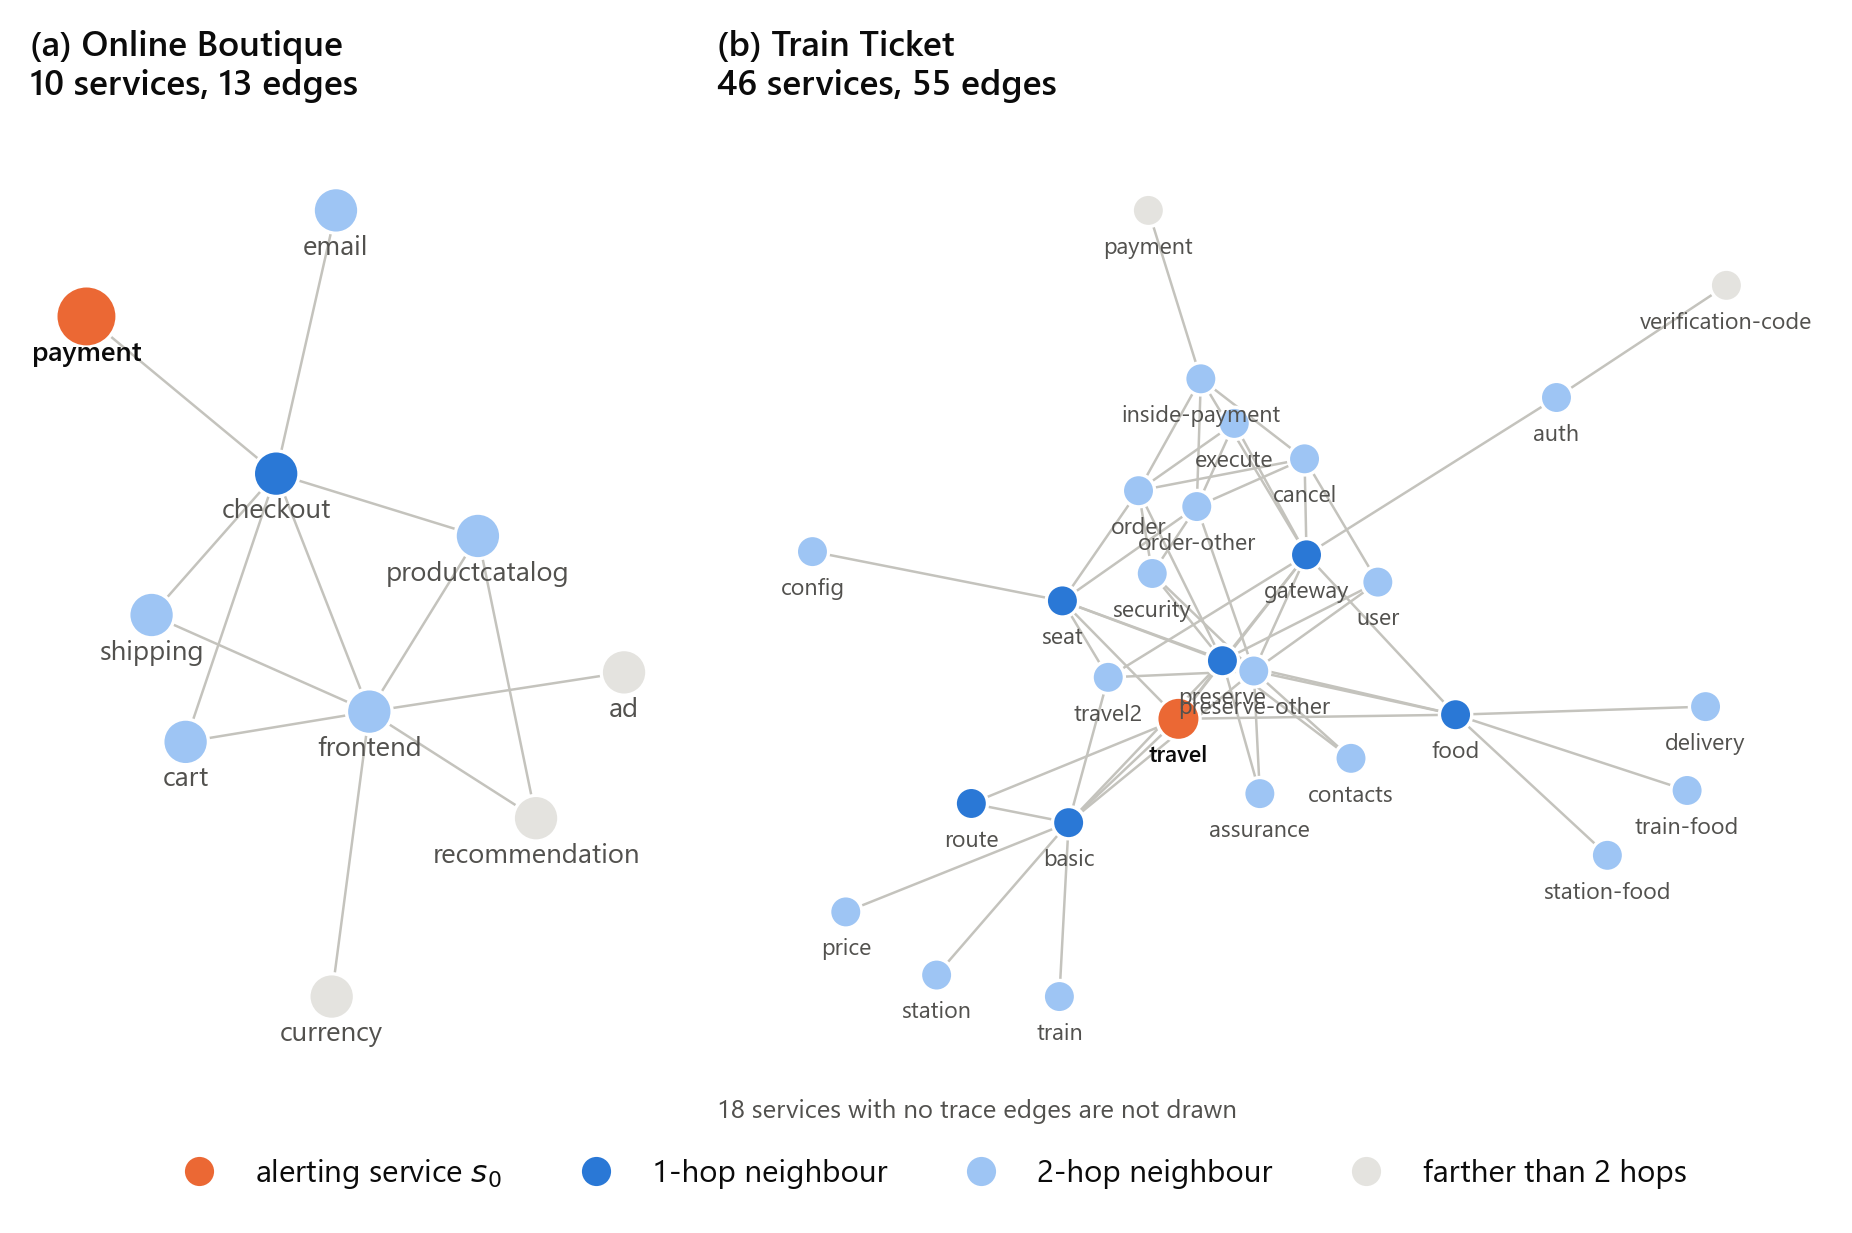
\includegraphics[width=\linewidth]{Images/C1/figures/ch2/h2.4-service-graph.png}
  \vspace{0.35cm}
  \caption[Đồ thị phụ thuộc service dựng từ trace của Nezha]{Đồ thị phụ thuộc service dựng từ trace của Nezha: (a)~OnlineBoutique (10 service, 13 cạnh) và (b)~TrainTicket (46 service, 55 cạnh), minh họa vùng mở rộng 1~hop và 2~hop quanh $s_0$.}
  \label{fig:ch2-service-graph}
\end{figure}

Ví dụ trên OnlineBoutique, khi \code{paymentservice} chậm, triệu chứng thường xuất hiện sớm ở các service gọi nó như \code{checkoutservice} (1~hop) và \code{frontend} (2~hop) trước khi thấy log lỗi tại chính \code{paymentservice}. Tuy nhiên, \textbf{gần trên đồ thị} không đồng nghĩa với \textbf{có quan hệ nhân quả}, và đồ thị chỉ phản ánh các đường gọi từng xuất hiện trong trace. Đề tài khai thác đồ thị cho hai nhiệm vụ: mở rộng ngữ cảnh truy xuất trong \CTAV{} (Mục~\ref{sec:ch4-c1}) và gom sự cố, lan truyền ngược trong tác tử \term{RCA}{RCA} (Mục~\ref{sec:ch4-rca}).

\subsubsection{Hợp nhất đa phương thức (\term{FusionScore}{Fusion Score}) và \term{RAG}{RAG} trong giám sát}
\label{sec:ch2-fusion}
\label{sec:ch2-rag}

\textbf{Retrieval-Augmented Generation} (\term{RAG}{RAG})~\cite{lewis2020rag} kết hợp bộ truy xuất với mô hình ngôn ngữ để đưa dữ liệu thời gian thực (log, span quanh cảnh báo) vào prompt thay vì để mô hình đoán từ tri thức tĩnh, giúp kết luận dẫn được về bằng chứng cụ thể. Tuy nhiên, truy xuất theo từ khóa đơn thuần (\term{BM25}{BM25}) dễ bỏ sót triệu chứng ở service lân cận không khớp từ khóa. \textbf{Truy xuất lai nhận biết topology} (\term{FusionScore}{Fusion Score}~\cite{icaetm2026}) giải quyết bằng cách gom ứng viên từ cả kênh \term{BM25}{BM25} lẫn các service trong bán kính $2$~hop, rồi xếp hạng theo tổ hợp tuyến tính của ba tín hiệu chuẩn hóa: mức khớp từ vựng ($\widehat{\text{BM25}}$), độ gần thời gian suy giảm theo hàm mũ quanh trung điểm cửa sổ $t_0$, và độ gần đồ thị $\text{GraphSim} = 1 / (1 + d_G)$.

Mặt trái của cơ chế hợp nhất này là khi cửa sổ thực chất bình thường, những sự kiện nền vô hại nhưng nằm rất sát $t_0$ hoặc gần trên đồ thị vẫn đạt điểm cao và lọt vào ngữ cảnh của LLM, dễ kích hoạt \term{ConfirmationBias}{thiên lệch xác nhận} (Mục~\ref{sec:ch2-thien-lech}). Công thức \term{FusionScore}{Fusion Score} đầy đủ, trọng số $(\alpha, \beta, \gamma)$ và cài đặt thành phần \comp{C1} được trình bày tại Mục~\ref{sec:ch4-c1}; ý tưởng liên quan dùng bằng chứng log/topology để cứu cửa sổ dưới ngưỡng metric được khảo sát qua cổng Rescue (\comp{C5}, chỉ là ablation) ở Mục~\ref{sec:ch4-detector}.

% -----------------------------------------------------------------------------
\subsection{LLM làm bộ thẩm định (LLM-as-a-Judge)}
\label{sec:ch2-judge}

Mục này giải thích cách một mô hình ngôn ngữ lớn được dùng để thẩm định cảnh báo, cách kiểm soát chi phí khi gọi nó, và các rủi ro về độ tin cậy mà phần đề xuất phải xử lý.

\subsubsection{LLM-as-a-Judge, đầu ra có cấu trúc và kiểm soát ngân sách}
\label{sec:ch2-prompt}
\label{sec:ch2-ngan-sach}

\textbf{LLM-as-a-Judge}~\cite{zheng2023judging} là cách dùng mô hình ngôn ngữ lớn để đánh giá hoặc phân loại đầu vào dựa trên tiêu chí cho trước. Trong vận hành hệ thống, LLM đọc trực tiếp log và thông điệp lỗi không cần huấn luyện lại, nhưng có ba hạn chế: độ trễ lớn, chi phí theo token và đầu ra không hoàn toàn tất định kể cả ở $\text{temperature} = 0$. Để tích hợp vào pipeline tự động, đầu ra phải bị ràng buộc theo \textbf{lược đồ JSON có cấu trúc} (nhãn phán quyết, mức ưu tiên, độ tin cậy, danh sách định danh bằng chứng hợp lệ, lý do và khuyến nghị) và được kiểm tra trước khi sử dụng.

Kết luận thô của judge chưa phải quyết định cuối mà đi qua một \textbf{chính sách quyết định}: chấp nhận cảnh báo, bác bỏ hoặc chuyển sang \code{manual\_review} khi thiếu bằng chứng hoặc dưới ngưỡng tin cậy — tương ứng nguyên lý phân loại có lựa chọn từ chối (\emph{reject option})~\cite{chow1970reject}. Để kiểm soát chi phí API dưới ràng buộc ngân sách $B$ lượt gọi theo thứ tự thời gian, cộng đồng thường dùng kiến trúc thẩm định theo tầng (\emph{cascade}, như FrugalGPT~\cite{chen2024frugalgpt}) kết hợp cơ chế bộ nhớ đệm (\emph{cache}) theo hàm băm của prompt để bảo đảm khả năng tái lập. Đặc tả lược đồ JSON, khóa cache \code{sha256}, mô hình cố định \code{gemini-2.5-flash} và các cơ chế định tuyến/chính sách của hệ thống được trình bày ở Mục~\ref{sec:ch4-policy}--\ref{sec:ch4-judge} và dùng trực tiếp cho chế độ demo ngoại tuyến ở Chương~\ref{ch:platform}.

\subsubsection{\term{ConfirmationBias}{Thiên lệch xác nhận}, hiệu chỉnh ngưỡng và nguồn gốc bằng chứng}
\label{sec:ch2-thien-lech}

\textbf{\term{ConfirmationBias}{Thiên lệch xác nhận}} (\emph{confirmation bias}) là xu hướng diễn giải bằng chứng theo hướng xác nhận giả định có sẵn; trên LLM, xu hướng đồng thuận với gợi ý trong prompt (\emph{sycophancy}) đã được ghi nhận rộng rãi~\cite{sharma2024sycophancy}. Khi prompt nêu rõ đang có cảnh báo và đính kèm bằng chứng sát thời điểm, judge dễ kết luận \code{true\_alert} ngay cả khi bằng chứng chỉ là hoạt động nền bình thường (minh họa ở Hình~\ref{fig:ch2-confirmation-bias}).

\begin{figure}[htbp]
  \centering
  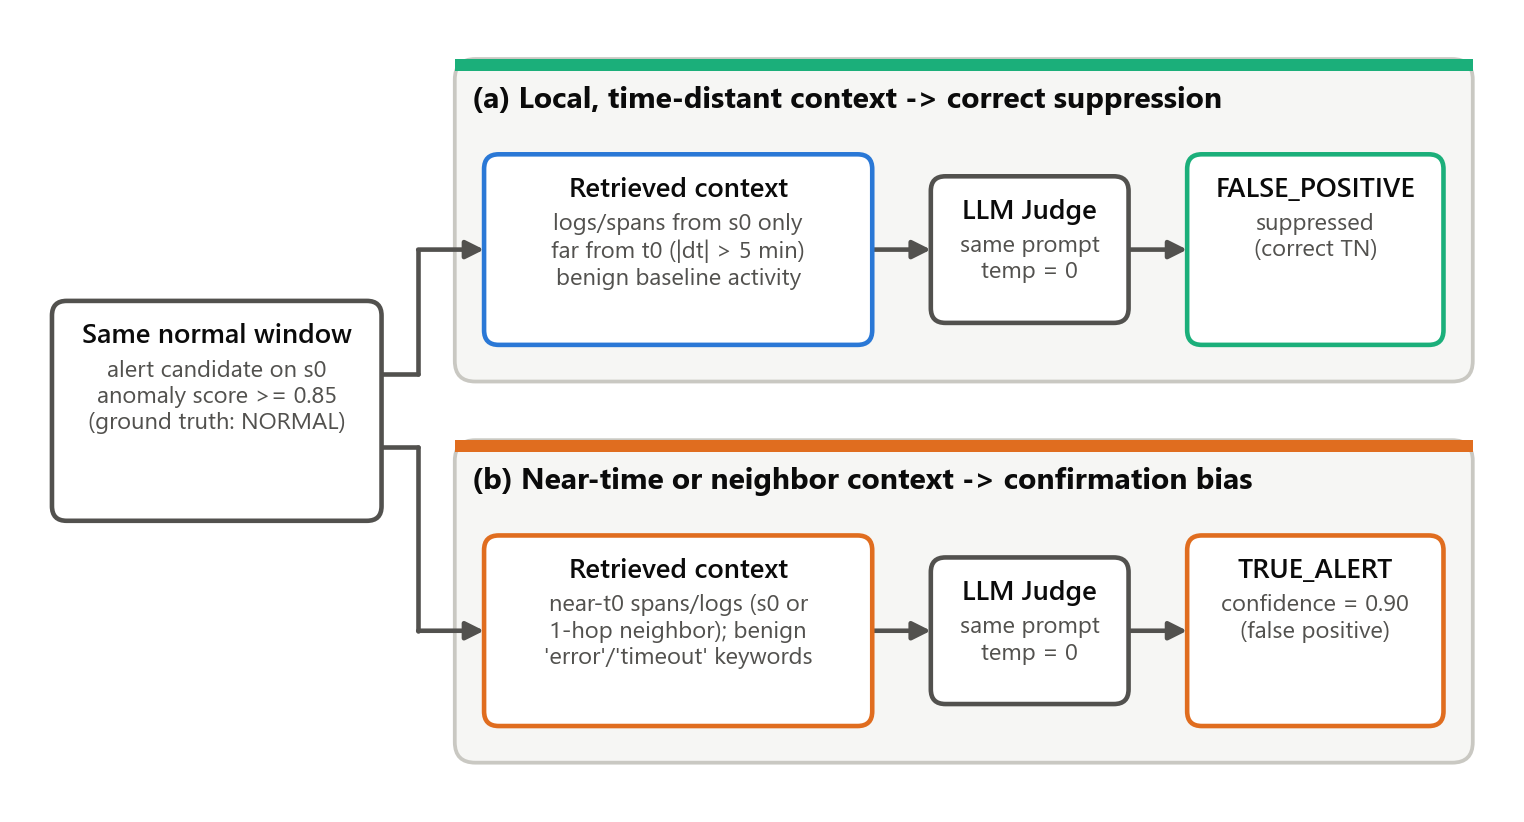
\includegraphics[width=\linewidth]{Images/C1/figures/ch2/h2.7-confirmation-bias.png}
  \vspace{0.35cm}
  \caption[Minh họa thiên lệch xác nhận của bộ thẩm định LLM]{\term{ConfirmationBias}{Thiên lệch xác nhận} của judge trên cùng một cửa sổ bình thường: (a)~ngữ cảnh xa thời điểm cảnh báo cho \code{false\_positive}; (b)~ngữ cảnh sát thời điểm hoặc từ lân cận dẫn tới \code{true\_alert} sai. \emph{(Nguồn: tác giả vẽ, có hỗ trợ AI.)}}
  \label{fig:ch2-confirmation-bias}
\end{figure}

\textbf{Hiệu chỉnh và nguồn gốc bằng chứng.} Một bộ phân loại được hiệu chỉnh tốt khi xác suất dự đoán khớp tần suất đúng thực tế~\cite{guo2017calibration}, nhưng độ tin cậy tự khai bằng lời của LLM thường co cụm ở vài mốc tròn và tự tin thái quá~\cite{xiong2024uncertainty}, buộc ngưỡng $\theta$ phải được chọn trên \splitname{val} thay vì hiểu theo nghĩa đen. Bên cạnh đó, \textbf{nguồn gốc bằng chứng} (\emph{provenance}) phân biệt bằng chứng thuộc chính service phát cảnh báo $s_0$ với bằng chứng từ láng giềng đồ thị. Đây là cơ sở lý thuyết của hai hướng thiết kế trong \CTAV{}: đặt ngưỡng bất đối xứng theo nguồn bằng chứng (\comp{C2}, đã loại sau kiểm định) và \textbf{neo bằng chứng bất thường tại $s_0$} theo phân vị nền đo từ \splitname{dev} (\comp{C3}, đang dùng — Mục~\ref{sec:ch4-policy}; bằng chứng cơ chế ở Mục~\ref{sec:ch5-h1}).

% -----------------------------------------------------------------------------
\subsection{Phân tích nguyên nhân gốc (\term{RCA}{RCA}) trên microservice}
\label{sec:ch2-rca}
\label{sec:ch2-gom}
\label{sec:ch2-lan-truyen}
\label{sec:ch2-bao-cao}

\textbf{Phân tích nguyên nhân gốc} (\emph{root cause analysis}, \term{RCA}{RCA}) nhằm xác định \textbf{service gốc} gây ra sự cố, tách biệt với các service chỉ chịu ảnh hưởng dây chuyền (\emph{cascade}). Khi một service lỗi, các service gọi nó (ngược chiều cạnh $u \to v$) thường chậm hoặc phát lỗi theo, tạo ra nhiều cảnh báo liên tiếp. Chuỗi xử lý \term{RCA}{RCA} tiêu chuẩn sau tầng thẩm định gồm ba bước: (1)~\textbf{gom cảnh báo thành sự cố (\emph{incident})} theo độ gần thời gian và tính liên thông trên đồ thị phụ thuộc; (2)~\textbf{lần ngược đồ thị gọi} để xếp hạng các service nghi vấn gốc (cần lưu ý giới hạn khi quan hệ gọi không đồng nghĩa nhân quả hoặc cảnh báo đầu vào bị thiếu); và (3)~\textbf{sinh báo cáo chẩn đoán có cấu trúc} (JSON) trích dẫn bằng chứng hợp lệ cho kỹ sư trực. Thuật toán gom nhóm, công thức bỏ phiếu lan truyền ngược 1 bước và bộ kiểm duyệt báo cáo cụ thể của tác tử \term{RCA}{RCA} được trình bày tại Mục~\ref{sec:ch4-rca}.

% -----------------------------------------------------------------------------
\subsection{Tiêu chí và phương pháp đánh giá}
\label{sec:ch2-danh-gia}

Mục này xác lập các thước đo hiệu năng và công cụ kiểm định thống kê dùng trong Chương~\ref{ch:thuc-nghiem}.

\subsubsection{Thước đo phân loại cảnh báo và định vị \term{RCA}{RCA}}
\label{sec:ch2-chi-so}
\label{sec:ch2-hitk}

Với bài toán thẩm định cảnh báo, mỗi cửa sổ được phân vào một trong bốn ô TP, FP, FN, TN và đánh giá bằng bốn chỉ số chuẩn: \textbf{Precision}, \textbf{Recall}, \textbf{F1} và \textbf{\term{FPR}{FPR}} ($\mathrm{FP}/(\mathrm{FP}+\mathrm{TN})$). Hai quy ước quan trọng được áp dụng xuyên suốt: (i)~Recall luôn tính trên \emph{toàn bộ} cửa sổ lỗi của split (kể cả cửa sổ bị detector bỏ sót) để tránh thổi phồng; và (ii)~vì dữ liệu mất cân bằng $1:135$, Precision và F1 rất nhạy với \term{FPR}{FPR} (như ví dụ Mục~\ref{sec:ch2-khoang-trong}), nên \term{FPR}{FPR} luôn được báo cáo tường minh bên cạnh số lần gọi LLM và chi phí token.

Với tác tử \term{RCA}{RCA}, mỗi sự cố có danh sách xếp hạng service; \textbf{\term{HitK}{Hit@k}} (dùng \term{HitK}{Hit@1} và \term{HitK}{Hit@3} ở mức service) đo tỷ lệ sự cố đơn lỗi mà service gốc nằm trong $k$ vị trí đầu (sự cố đa lỗi nhập nhằng bị loại khỏi \term{HitK}{Hit@k} và báo riêng). Mức nén cảnh báo được đo bằng \textbf{Alert Reduction Ratio} (\term{ARR}{ARR}):
\begin{equation}
  \mathrm{ARR} = 1 - \frac{\text{số incident}}{\text{số cảnh báo}}.
  \label{eq:ch2-arr}
\end{equation}
Baseline định vị là xếp hạng theo điểm bất thường cực đại trong sự cố; ngoài ra tỷ lệ báo cáo JSON hợp lệ cũng được theo dõi (Mục~\ref{sec:ch5-rca}).

\subsubsection{Bootstrap CI và kiểm định McNemar}
\label{sec:ch2-thong-ke}

Do số cửa sổ lỗi mỗi split chỉ ở mức vài trăm, đề tài dùng hai công cụ phi tham số (mức ý nghĩa $\alpha = 0{,}05$, hai phía) để tách tín hiệu khỏi nhiễu:
\begin{itemize}[label=--]
  \item \textbf{Bootstrap ghép cặp (CI95)}~\cite{efron1993bootstrap}: lấy mẫu lại có hoàn lại $N$ cửa sổ $1.000$ lần (\code{seed = 42}) đồng thời cho hai phương pháp $A$ và $B$ để tính khoảng tin cậy 95\% phân vị của hiệu $\Delta = \text{chỉ số}(A) - \text{chỉ số}(B)$; nếu CI95 chứa $0$ thì chưa đủ bằng chứng kết luận khác biệt.
  \item \textbf{Kiểm định McNemar chính xác}~\cite{mcnemar1947note}: so sánh hai bộ phân loại trên cùng tập cửa sổ dựa trên số ca bất đồng ($b$: $A$ đúng, $B$ sai; $c$: $A$ sai, $B$ đúng), với giá trị $p$ hai phía:
  \begin{equation}
    n = b + c, \qquad
    p = \min\!\left(1,\; 2 \sum_{i=0}^{\min(b, c)} \binom{n}{i} 0{,}5^n\right).
    \label{eq:ch2-mcnemar}
  \end{equation}
\end{itemize}
\hyp{H2} là giả thuyết chính; với các giả thuyết phụ, $p$ được báo thô không hiệu chỉnh đa so sánh (Mục~\ref{sec:ch7-hop-le}). Độ dao động lặp lại của judge được đo riêng bằng \code{repeat} $\in \{0, 1, 2\}$ trên mẫu 200 cửa sổ (Mục~\ref{sec:ch5-repeat}).

% -----------------------------------------------------------------------------
\subsection{Giả thuyết nghiên cứu và đăng ký trước}
\label{sec:ch2-dang-ky}

\textbf{Đăng ký trước} (\emph{pre-registration}) ghi cố định giả thuyết, phép so sánh và tiêu chí bác bỏ \emph{trước} khi chạy trên tập kiểm định để ngăn tinh chỉnh hậu nghiệm. Đề tài tuân thủ ba quy tắc: mọi chọn lọc tham số chỉ thực hiện trên \splitname{dev} và \splitname{val}; tập \splitname{test} chỉ chạy đúng một lần sau khi khóa bản đăng ký \hyp{H0}--\hyp{H5} (ngày 14/11/2026, với \hyp{H2} là giả thuyết chính có biên $\delta = 0{,}05$, \hyp{H1} chỉ chạy trên mẫu cố định của \splitname{val}); mọi sai lệch phát sinh đều được ghi nhận minh bạch thay vì sửa ngược. Bảng đầy đủ tiêu chí \hyp{H0}--\hyp{H5} đặt tại Bảng~\ref{tab:h0-h5} (Mục~\ref{sec:ch5-hypotheses}).

% -----------------------------------------------------------------------------
\subsection{Công nghệ nền tảng}
\label{sec:ch2-cong-nghe}

Bảng~\ref{tab:ch2-cong-nghe} tóm tắt các công nghệ hiện thực hệ thống cùng vai trò và lý do lựa chọn (cách lắp ráp thành hệ thống hoàn chỉnh trình bày tại Mục~\ref{sec:ch4-impl}). Đề tài cố định một mô hình API duy nhất (\code{gemini-2.5-flash}, $\text{temperature} = 0$, qua cache) cho mọi phương pháp để loại trừ nhiễu đổi mô hình, đồng thời tách vai trò lưu trữ giữa ClickHouse (dữ liệu sự kiện cột phục vụ truy vấn tổng hợp) và PostgreSQL (dữ liệu quan hệ cho sự cố và báo cáo chẩn đoán).

\begin{table}[H]
  \centering
  \caption{Công nghệ nền tảng: vai trò trong hệ và lý do chọn.}
  \label{tab:ch2-cong-nghe}
  \tblfont
  \tblsetup
  \begin{tabularx}{\linewidth}{|>{\raggedright\arraybackslash}p{3.4cm}|>{\raggedright\arraybackslash}p{1.9cm}|Y|Y|}
    \hline
    \rowcolor{gray!15}
    \textbf{Công nghệ} & \textbf{Phiên bản} & \textbf{Vai trò trong hệ} & \textbf{Lý do chọn} \\
    \hline
    Python~\cite{python2026docs} & $\ge 3.11$ & Ngôn ngữ của mọi service, harness thực nghiệm và script & Hệ sinh thái khoa học dữ liệu; một ngôn ngữ cho cả thực nghiệm lẫn hệ thống \\
    \hline
    scikit-learn~\cite{pedregosa2011sklearn} & $\ge 1.4$ & Isolation Forest của bộ phát hiện & Cài đặt chuẩn, có kiểm thử, tham số rõ ràng \\
    \hline
    Gemini API~\cite{google2026gemini} (\code{gemini-2.5-flash}) & REST \code{v1beta} & Judge của \CTAV{} và bộ tóm tắt của tác tử \term{RCA}{RCA} & Một model API cố định cho mọi phương pháp; trả JSON; chi phí thấp cho hàng chục nghìn lần gọi \\
    \hline
    ClickHouse~\cite{clickhouse2026docs} & 24.3 & Lưu mọi kết luận của judge cùng bằng chứng, phục vụ truy vấn phân tích & Cơ sở dữ liệu cột, truy vấn tổng hợp nhanh trên hàng chục nghìn candidate \\
    \hline
    PostgreSQL~\cite{postgresql2026docs} & 16 & Lưu incident và báo cáo chẩn đoán & Dữ liệu quan hệ, có ràng buộc, cần tính toàn vẹn \\
    \hline
    FastAPI~\cite{fastapi2026docs} & $\ge 0.110$ & API chỉ đọc cho dashboard & Kiểu dữ liệu tường minh qua Pydantic, tài liệu API tự sinh \\
    \hline
    React~\cite{react2026docs} và Vite~\cite{vite2026docs} & React 19, Vite 8 & Dashboard năm màn hình & Giao diện thành phần; tách gói theo màn hình, hỗ trợ chạy tĩnh ngoại tuyến \\
    \hline
    Docker Compose~\cite{docker2026compose} & --- & Triển khai toàn hệ bằng một lệnh, hai profile \code{dev} và \code{full} & Tái lập môi trường trên máy khác, kể cả lúc demo \\
    \hline
  \end{tabularx}
\end{table}

% -----------------------------------------------------------------------------
\subsection{Kết chương}
\label{sec:ch2-ket-chuong}

Chương này đã xác lập hệ thống kiến thức và công nghệ nền tảng theo đúng luồng xử lý của đề tài: đơn vị cửa sổ $60\,\text{s}$ và bộ dữ liệu Nezha; bộ phát hiện Isolation Forest cùng khoảng trống ngữ nghĩa; truy xuất bằng chứng \term{BM25}{BM25}, đồ thị phụ thuộc service và nguyên lý \term{RAG}{RAG} lai; cơ chế \emph{LLM-as-a-Judge}, \term{ConfirmationBias}{thiên lệch xác nhận} và hiệu chỉnh theo nguồn gốc bằng chứng; bài toán \term{RCA}{RCA} trên microservice; cùng khung đánh giá thống kê (bootstrap CI, McNemar, đăng ký trước) và ngăn xếp công nghệ hiện thực. Mọi thành phần đề xuất ở Chương~\ref{ch:de-xuat}, mọi phép kiểm định ở Chương~\ref{ch:thuc-nghiem} và toàn bộ platform trình diễn ở Chương~\ref{ch:platform} đều dựa trực tiếp trên các khái niệm này, cho thấy nền tảng lý thuyết và kỹ thuật đã đầy đủ để chuyển sang khảo sát công trình liên quan và thiết kế hệ thống.
